%%%%%%%%%%%%%%%%%%%%%
%                                              %
%                 Experiment M-5               %
%            Conservation of Energy            %
%                                              %
%%%%%%%%%%%%%%%%%%%%%

\labChapter{M}{Conservation of Energy with Glider on Tilted Air Track}
\label{lab:M5}

% Introduction
%\section{Introduction}
% Background
\section{Background}

\textbf{Energy cannot be created nor destroyed.}  All that can really happen is a change in its form. We shall consider the conservation of mechanical energy, in particular, the sum of the kinetic energy and potential energy of a mass.  The kinetic energy is due to the motion of the mass and the potential energy is due to the relative position of the mass in the earth's gravitational field.  This total mechanical energy can only change if nonconservative forces are acting on any part of the system.  We will examine the exchange of kinetic and potential energy and the conservation of mechanical energy under the presumption of no nonconservative forces acting.  If the mechanical energy is not conserved we will attempt to determine potential sources of nonconservative work being done that would change the mechanical energy.





The \textbf{work} done by a force acting on a mass is the magnitude of the force acting in the direction of motion times the distance the mass moves.  Work is only done when the mass moves.  (In other words, you can push as hard as you like on a brick wall, but if the wall doesn't move, you didn't do any work!)  Assume for the moment that we have a mass $m$ moving on a frictionless, horizontal surface.  Assume a force acts on the mass from the position $x = 0$ to $x = x_1$ as illustrated in Fig.~\ref{M05Fig01}.  At position $x = 0$ it is moving with a velocity $v_{0}$ and at $x = x_1$ the velocity is $v_1$.

\begin{figure}
  \begin{center}
    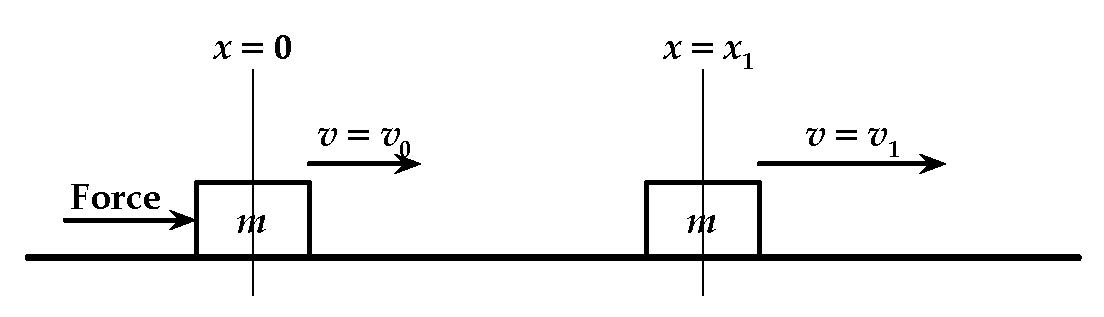
\includegraphics[width=5.0in]{Experiment04Figures/Figure01.pdf}
  \end{center}
  \caption{Explanation of the variables needed to calculate the amount of work done on a mass}
  \label{M05Fig01}  % the \label command comes AFTER the caption
\end{figure}

The work done by the force is $W_F = \vec{F} \cdot \vec{x_1}$.  Using Newton's second law it can easily be shown that the work done by the force changes a quantity we call the \textsl{kinetic energy}, $K = \nicefrac{1}{2} m v^2$.  Using the example illustrated in Fig.~\ref{M05Fig01},
\[
\vec{F} \cdot (\vec{x}_1 - \vec{0}) =
\frac{1}{2} m \,{v_1}^2 -  \frac{1}{2} m \,{v_0}^{2}.
\]
In this case, the force is acting in the direction of the motion and thereby increases the kinetic energy.  If the force were acting in the direction opposite to the motion, then the kinetic energy would be decreased.  If friction were present, it would act in the direction opposite to the direction of motion and thereby reduce the kinetic energy.  In this simple analysis, we have made no assumption as to the nature of the force.

A force like friction is a non-conservative force.  The work done by it not only depends upon the path the mass takes but is also not completely recoverable.  However, the work done on a mass by a conservative force can be completely returned to the mass as mechanical energy.  Thus work done by a conservative force can be represented by a potential energy function and depends only on the end points of the process. The gravitational force is a conservative force and is assumed constant in the vicinity of the surface of the earth.  The potential energy function is merely the work done by gravity on the way up or the way down and is equal to the gravitational force (the weight $m g$) times the change in height, $h$.  The gravitational potential energy, $U$, is given by
\[
U = m g h.
\]
The work done by this conservative force, like all conservative forces, only depends on the end-points of the path.  The gravitational potential energy is a relative quantity, i.e.\ it is a change in energy because of a change in elevation.  Thus we can choose a zero level arbitrarily.

If there are no non-conservative forces acting, then a mass moving only under the influence of gravity merely exchanges its kinetic and potential energy while the total energy remains constant.  For a mass stationary at some height, $h$, above the ground, all of its energy is potential energy of value $mgh$ with respect to the ground.  As the mass begins to fall under the influence of gravity, it loses $U$ and gains $K$  When it reaches the ground, the $U$ is zero with respect to the ground and the $K$ is a maximum, equal to the original $U$ at the top.  If the mass were a roller coaster, the coaster could climb back up to its original height where all the energy would be $U$ at which point it would momentarily stop, i.e.\ no $K$.  This assumes that neither friction nor any other nonconservative force is acting.  In general, we have
\[
\mbox{Work done by non-conservative Forces} = W_{N.C.} = \Delta K + \Delta U.
\]
If there are no non-conservative forces acting, then
\[
\Delta K + \Delta U = 0.
\]

In this experiment, we will use an air track to provide a nearly frictionless surface.  The track will be tilted at a measurable angle.  A glider will be released from rest at the top of the track and allowed to slide down and collide with a spring at the bottom. If the force of the spring on the glider is conservative, then the kinetic energy of the glider at the bottom is converted to potential energy in the compressed spring.  This potential energy is given back to the glider in the form of kinetic energy as the spring expands.  The glider bounces off and goes back up the track to its original height where the energy is again all $U$. If no energy is lost in the collision at the bottom, we say that the collision is completely elastic, implying that the forces involved in the collision are conservative.  After the collision, the glider will rebound up the track.  Getting back to its original height therefore implies no mechanical energy is lost during the entire path.  If it does not, we have to look for an energy loss mechanism and some non-conservative forces acting.

The change in height from the top to the bottom is measured allowing the change in $U$ to be calculated.  We will set the zero level for the potential energy at the bottom of track, at the position, $s_0$, in Fig.~\ref{M05Fig02}.

A measurement of the transit time from the top to the bottom will allow the calculation of the velocity at the bottom and therefore the $K$ at the bottom.  Finally, measuring the maximum height achieved on the rebound will yield a second value of $U$

The $K$ at the bottom of the track can be determined by measuring the average velocity from the release point at the top, $s_1$, to the collision point at the bottom, $s_0$, and then using Equation 1.  From a measurement of the transit time from $s_1$ to $s_0$, the velocity of the glider at the moment of collision at the bottom, $v_b$, can be determined by using the definition of average velocity, $v_{avg}$, thus:
\[
\frac{\Delta s}{\Delta t}  = v_{\mbox{avg}} = \frac{1}{2} (v_{b}+v_1)
\]
where the initial velocity, $v_1 = 0$, $\Delta s$ is the distance traveled down the track, and $\Delta t$ is the transit time of travel.

Rearranging terms we have the velocity at the bottom in terms of measurable quantities
\begin{equation}
  v_b = 2 v_{\mbox{avg}} = 2 (\Delta s / \Delta t).
\end{equation}
Using the definition of $K$, the $K$ at the bottom is then
\begin{equation}
  K_b = \frac{1}{2} m\, {v_b}^2.
\end{equation}

In order to calculate the potential energy, $U$ at any point, along the track we must determine the change in height between $s_1$ and $s_0$.  The potential energy at any position along the track is measured with respect to the collision point at the bottom, $s_0$, which is arbitrarily assigned a value of zero potential energy.  The $U$ is given by the weight of the glider, $mg$, times the change in vertical height.

Fig.~\ref{M05Fig02} is a simplified diagram of the inclined track. The distance $s$ is measured along the track by the scale attached to the side of the track.  The change in elevation, $\Delta h$, of any other point $s$ along the track can now be determined from the distance $s$ and the incline angle of track, $\theta$.  The incline of the track is produced by placing a spacer of known height under a leg at one end.  With the height of the spacer and the distance between the legs, $D$, the angle can be calculated (See Fig.~\ref{M05Fig03}).

\begin{figure}
  \begin{center}
    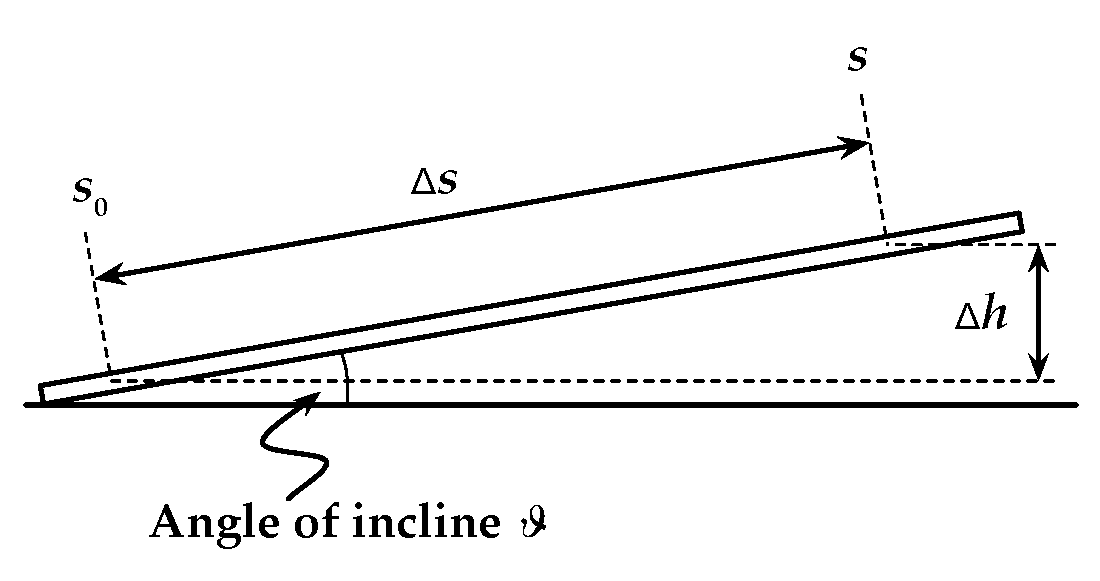
\includegraphics[width=4.5in]{Experiment04Figures/Figure02.pdf}
  \end{center}
  \caption{Schematic Drawing explaining the relationship between the track election $\Delta h$ and the distance $\Delta s$ for Experiment M-\ref{lab:M5}.}
  \label{M05Fig02}
\end{figure}

At $s_0$, $U_{b} = 0$, therefore $U_{s} = mg\, \Delta h = mg\, \Delta s \sin(\theta)$.
Referring to Fig.~\ref{M05Fig03}, the $\tan(\theta) = (\mbox{height of the spacer}) / (\mbox{distance between legs})$ or
\[
\tan(\theta) = \frac{H}{D}.
\]
With the very small angles of incline being used, we can safely assume that
\[
\tan(\theta) \sim \sin(\theta),
\]
therefore the potential energy, $U$, at some position, $s$, along the track is finally given by measurable quantities as
\begin{equation}
  U_s = mg \, \Delta s \frac{H}{D}.
\end{equation}

% Testing your Understanding
\section{Experimental Procedure}

\begin{figure}
  \begin{center}
    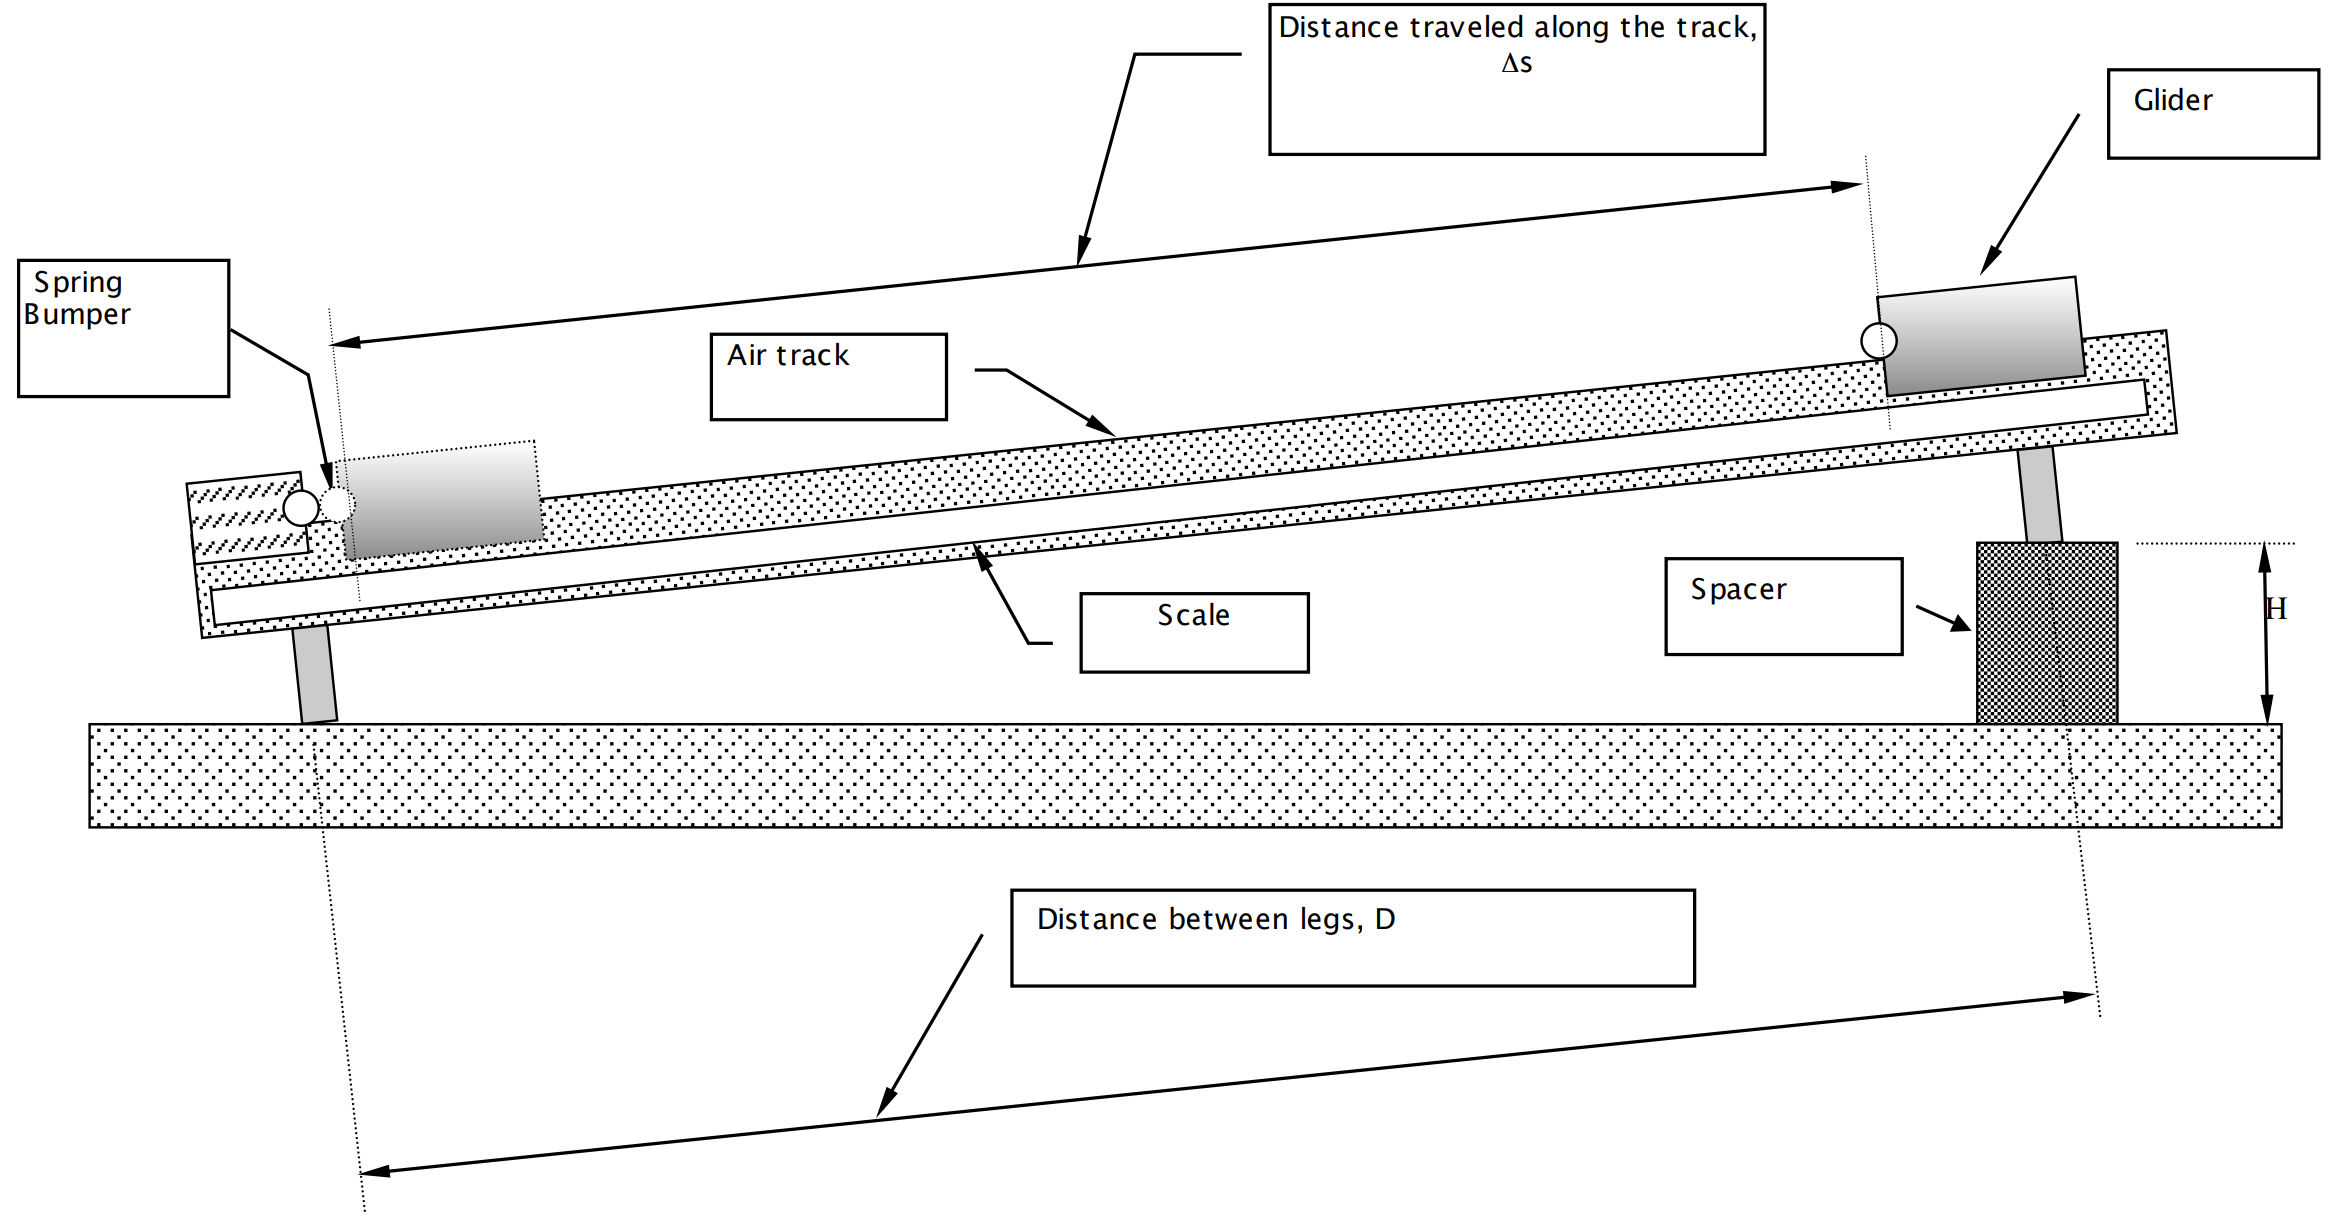
\includegraphics[width=5.8in]{Fall/Experiment04Figures/M04_fig2.png}
  \end{center}
  \caption{Experimental setup for Experiment M-\ref{lab:M5}.}
  \label{M05Fig03}
\end{figure}

\begin{itemize}
\item[$\triangleright$] Turn on the air and allow it to run a couple of minutes before proceeding.  It is very important that the track is clean and free of dirt.  This will prevent any damage to the very expensive air track and will keep friction to an absolute minimum.  Do not put a glider on the track without air flowing.
\item[$\triangleright$] Measure and record the mass of both a large and a small glider.
\item[$\triangleright$] Without the spacer present and the air track resting directly on the tabletop, place one of the gliders on the track and note any preferential drift of the glider.  Adjust the height of the single leg until the air track is level, as indicated by no preferential drift.  Check both orientations of the glider on the track to check if the car is asymmetric and has a significant preferential drift on an otherwise level track.  If this occurs, use another glider.
\item[$\triangleright$] Measure and record the distance $D$.  This is the center-to-center distance between the legs.
\item[$\triangleright$] Measure and record the heights $H$, of each of the two spacers.  Use a Vernier caliper for maximum accuracy. See the instructions at Fig.~\ref{VernierFig02} for using the Vernier caliper.
\item[$\triangleright$] Four cases will be performed, two gliders for two spacers.  Determine a convenient point on the glider to use with the scale attached on the side of track.  It doesn't matter what point you choose, only that you use the same point for all $s$ determinations for that glider.  A convenient point is the lower front or rear corner of the glider since it will be very close to the scale.
\item[$\triangleright$] For each case, perform the following steps and record the data appropriately in your spreadsheet:
  \begin{enumerate}
  \item Raise the single leg side of the track by placing a spacer under the knob.
  \item Place the glider at the bottom of the track resting against the bumper. Record $s_0$. (Note: With the car at this position, the red light on the bottom photogate should be lit. Moving the glider to the right the slightest distance should put the light out. If this is not the case, adjust the position of the photogate.)
  \item Next, place the glider near the top of the track. Move it slowly as you approach the top photogate. Stop the glider at the exact location when the red light comes on. Record $s_1$.
  \item Before you take the recorded data in the next step, take some practice runs. Your subsequent data will be much improved by your training!  %Set the photogate timer to pulse mode. 
  \begin{itemize}
      \item Position the glider so it is blocking the top photogate and the red light is on. Place one finger on the track in front of the glider and gently push the glider to the right until the red light on the photogate just goes out.
      \item Press record in \textbf{Capstone} to start the timer. \textit{NOTE: }\textbf{Capstone} may take a few seconds to start displaying times, once it's going, it will display the time whenever a photogate beam is broken; the time at the higher (start) photogate $t_1$ as well as the time at the lower (end) photogate $t_0$. Total transit time $\Delta t$ will be the the difference of the start and end times.
      \item Release the glider by quickly pulling your finger away from the track. After the glider bounces off the lower bumper, you can calculate the time of travel from top to bottom $\Delta t$.
  \end{itemize} 
    \item For each of the five trials, release the glider from the $s_1$ point and measure and record the following:
    \begin{itemize}
    \item The transit time $\Delta t$ from release at the top to the collision at the bottom.  Release the glider very carefully to insure that the initial velocity is zero.
    \item Allowing the glider to rebound off the bumper, record the rebound position $s_2$.  As the glider slows to a stop, capture the glider by gently pressing your finger near a lower corner of the glider just as it comes to a stop and then read $s_2$ off the scale.  Use the same point on the glider to read $s_2$ that you used to read $s_1$ and $s_0$.
    \end{itemize}
  \end{enumerate}
\end {itemize}

\textbf{Data Table:}

\begin{itemize}
\item[$\triangleright$] Create a table of the common data including the masses of the gliders, the distance $D$ between the legs of the air track and the heights of the two spacers.

\item[$\triangleright$] Create a table for each case with rows for each of the five trials including:
  \begin{itemize}
  \item The starting point $s_1$ at the top
  \item The stopping point $s_0$ at the bottom
  \item Start time at the top $t_1$
  \item End time at the bottom $t_0$
  \item The time $\Delta t$ (s) for each of the five trials
  \item The rebound position $s_2$ at the top
  \item Initial distance, $\Delta s_1=s_1-s_0$
  \item Initial potential energy at top, $U_{\mbox{top}}$
  \item The speed at the bottom, $v_{\mbox{b}}$
  \item Kinetic energy at the bottom, $K_{\mbox{b}}$
  \item Final distance, $\Delta s_2=s_2-s_0$
  \item Final potential energy at the rebound position, $U_{\mbox{rebound}}$
  \end{itemize}


\item[$\triangleright$] Create a summary table of the analysis with a row for each case including the following data:
  \begin{itemize}
  \item The average and standard deviation of the time, $\Delta t$, for the five trials
  \item The average and standard deviation of the speed at the bottom, $v_{\mbox{b}}$
  \item The average and standard deviation of the kinetic energy at the bottom, $K_{\mbox{b}}$
  \item The average and standard deviation of the final potential energy at the rebound position, $U_{\mbox{rebound}}$
  \item \% change from initial potential energy to kinetic energy at the bottom
  \item \% change from initial potential energy to final potential energy
  \end{itemize}

Calculate the following:
\begin{itemize}
\item[$\triangleright$] For each case, calculate the initial potential energy at $s_1$. Average the transit times, $\Delta t$, and calculate the velocity $v_b$ and the $K_b$.
\item[$\triangleright$] For each case, average the rebound position, $s_2$. Using this averaged value, calculate the final $U_2$.
\item[$\triangleright$] Calculate the percent change in mechanical energy from the top to the bottom.
\item[$\triangleright$] Calculate the percent change in mechanical energy from the initial release point $s_1$ to the final rebound point $s_2$.
\end{itemize}

\end{itemize}




\section{Post-Lab Submission --- Interpretation of Results}


\begin{itemize}
    \item Make sure to submit your finalized data table (Excel sheet)
    \item Arguing your responses with your data $\pm$ standard deviation:
    \begin{itemize}
        \item Is energy conserved between top and bottom?
        \item Is energy conserved between top/bottom and rebound?
    \end{itemize}
    \item Why is there a difference in energy conservation between the top/bottom and top/bottom/rebound?
    \item Uncertainties: 
    \begin{itemize}
        \item What is the precision of your equipment?
        \item What are the effects of measured uncertainties on your determined energies?
        \item What are possible systematic errors for today's experiments?
        \item How could one gain energy between top and bottom?
    \end{itemize}
\end{itemize}


